\documentclass[handout]{beamer}
\usepackage[utf8]{inputenc}

\usepackage{natbib}  %havard referencing
\bibliographystyle{agsm}
\usepackage{xcolor}
\usepackage[tikz]{bclogo}
\usepackage[framemethod=tikz]{mdframed}
\usepackage{lipsum}
\usepackage{tikz,lipsum,lmodern}
\usepackage[most]{tcolorbox}
\usepackage{caption}
\usepackage{etoolbox}
\AtBeginDocument{\patchcmd{\label}{\strut}{}{}{}}
\usepackage{amsmath}
\usepackage{amssymb}
\usepackage[ruled,vlined]{algorithm2e}
\usepackage{amsthm}
\usepackage{amsfonts}
\usepackage{graphicx}
\usepackage{amsmath}
\usepackage{amssymb}
\usepackage{amsthm}
\usepackage{amsfonts}
\usepackage{xspace}
\usepackage{mathtools}
\usepackage[noend]{algpseudocode}
\usepackage{color}
\usepackage{tikz}
\usetikzlibrary{arrows}
\usepackage{xmpmulti}
\usepackage{svg}

\mode<presentation>
{
  \usetheme{Madrid}      % or try Darmstadt, Madrid, Warsaw, ...
  \usecolortheme{default} % or try albatross, beaver, crane, ...
  \usefonttheme{default}  % or try serif, structurebold, ...
  \setbeamertemplate{navigation symbols}{}
  \setbeamertemplate{caption}[numbered]
} 


\usepackage[english]{babel}
\title[Scheduling of Ticket Inspectors on ICEs]{Scheduling of Ticket Inspectors 
in Deutsche Bahn Inter-City Express Trains}
\author[May, Nguyen \& Abrams]{Nathan May \inst{1} \and Hai Nguyen \inst{2} \and 
Ruby Abrams \inst{3}}
\institute[]{\inst{1} Department of Mathematics, Washington State University, U.S.A. \and %
             \inst{2} School of Computer Science, University of Birmingham, U.K. \and
             \inst{3} Department of Mathematics, University of Arizona, U.S.A.}

\date[G-RIPS 2019]{G-RIPS 2019\\
Zuse Institut Berlin, Germany\\
August 15, 2019}

\begin{document}

\begin{frame}
  \titlepage
\end{frame}

\begin{frame}{Outline}
\small 
  \tableofcontents
\end{frame}


\section{Motivations}

\begin{frame}{Motivations}
\begin{itemize}
    \item  Currently the staffs on the ICEs stay on-board for the whole route to inspect passenger tickets.
    \item The number of passengers leaving
    and new passengers joining the train at some stop is usually 
    \textbf{relatively small}.
    \item \textbf{Inefficient} to have inspectors stay on-board all the time as many passengers might be inspected twice or more.
\end{itemize}

\begin{tcolorbox}[colback=yellow!5!white,colframe=yellow!75!black]
We try to formulate an alternative model, where the ticket inspectors
join the train only for a short part of the route while maximising the number
of passenger tickets inspected.
\end{tcolorbox}
\end{frame}

\section{The Ticket Inspection Scheduling Problem}

% Ruby
\begin{frame}{The Ticket Inspection Scheduling Problem}

%Input box
\begin{tcolorbox}[colback=blue!5!white,colframe=blue!75!black,title=Input]
  \begin{itemize}
    \item Number of inspectors \pause
    \item Depot station for each inspector (also called base) \pause
    \item Maximum number of working hours for each inspector \pause
    \item Maximum number of inspectors allowed to work\pause
    \item Train timetable \& train statistics for a specific day\pause
\end{itemize}
\end{tcolorbox}

%output box
\begin{tcolorbox}[colback=yellow!5!white,colframe=yellow!75!black,title=Output]
  A day-long working schedule for each inspector 
in order to maximise the number of passengers inspected 
on that day.
\end{tcolorbox}
\end{frame}

\section{A Brief Literature Review}
% Ruby
\begin{frame}{Previous Work: Game-Theoretic Approach\footnote{Image source: Internet}}

 \begin{figure}[ht]
        \begin{minipage}[b]{0.45\linewidth}
            \centering
            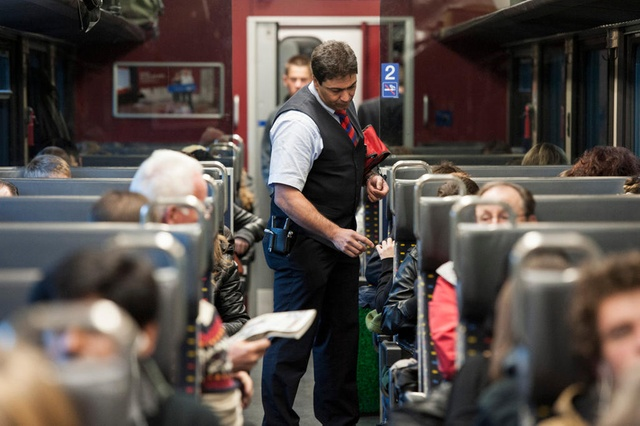
\includegraphics[width=.6\textwidth]{inspector.jpg}
            \caption*{Inspectors as Leader}
        \end{minipage}
        \hspace{0.5cm}
        \begin{minipage}[b]{0.45\linewidth}
            \centering
            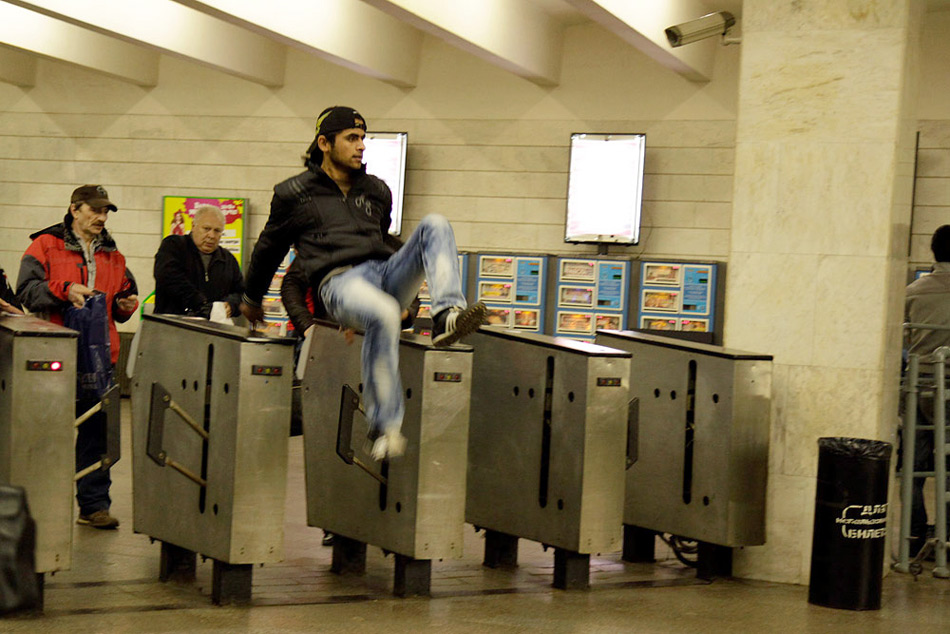
\includegraphics[width=.6\textwidth]{fare_evader.jpg}
            \caption*{Fare evaders as Followers}
        \end{minipage}
    \end{figure}
    
\begin{itemize}
    %\item Stackelberg strategies
    \item \cite{yin_jiang_tambe_kiekintveld_leyton-brown_sandholm_sullivan_2012} considered this model for the 
    Los Angeles transit systems (via a bi-level programming problem).
    \item Improved further by \cite{jiang_yin_johnson_tambe_kiekintveld_leyton-brown_sandholm_2012} 
    upon \textbf{history encoding} and \textbf{schedule regularisation} .
    \item \cite{mastersthesis} stated that the inspection scheduling is \textbf{not} a well studied problem.
\end{itemize}
\end{frame}


\begin{frame}{How is our work different?}

\begin{minipage}[t]{0.48\linewidth}
\begin{tcolorbox}[colback=yellow!5!white,colframe=yellow!75!black,title=Previous Work]
\begin{itemize}
    \item Maximise revenue (fine and ticket sale)
    \item Inspectors vs fare evader
    \item Available passenger information
    \item on-train and on-station inspections
\end{itemize}\end{tcolorbox}
\end{minipage}%
\hfill%
\begin{minipage}[t]{0.48\linewidth}
\begin{tcolorbox}[colback=blue!5!white,colframe=blue!75!black,title=Our Work]
\begin{itemize}
    \item Maximise number of passenger inspected
    \item Inspectors and passengers
     \item No waiting passenger information
         \item on-train inspection 
\end{itemize}
\end{tcolorbox}
\end{minipage}
\end{frame}


\section{Mathematical Model}

% Hai
\begin{frame}{How do we approach the problem?}
\begin{figure}
    \centering
    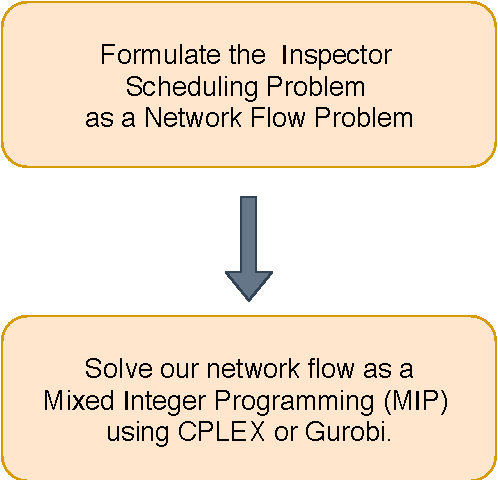
\includegraphics[scale=.7]{steps.pdf}
\end{figure}
\end{frame}

\begin{frame}{Our Assumptions}
    \begin{itemize}
        \item All passengers on a train 
        are \textbf{equally likely} to be inspected.
        \item All inspectors have the same \textbf{inspection rate} (i.e., 
        \#passengers inspected per minute)
        \item We have passenger route information (we don't)
        \item Inspectors do not have fixed starting/ending times
        \item \textbf{Not} all inspectors will be required to work on a specific day
    \end{itemize}
\end{frame}

\begin{frame}
  \vfill
  \centering
  \begin{beamercolorbox}[sep=8pt,center,shadow=true,rounded=true]{title}
    \usebeamerfont{title} Network Representation,\\
    Constraints and Objective Function \par%
  \end{beamercolorbox}
  \vfill
  \end{frame}
  
% Hai
\begin{frame}{Network Representation: Driving Edges}
\begin{figure}
    \centering
    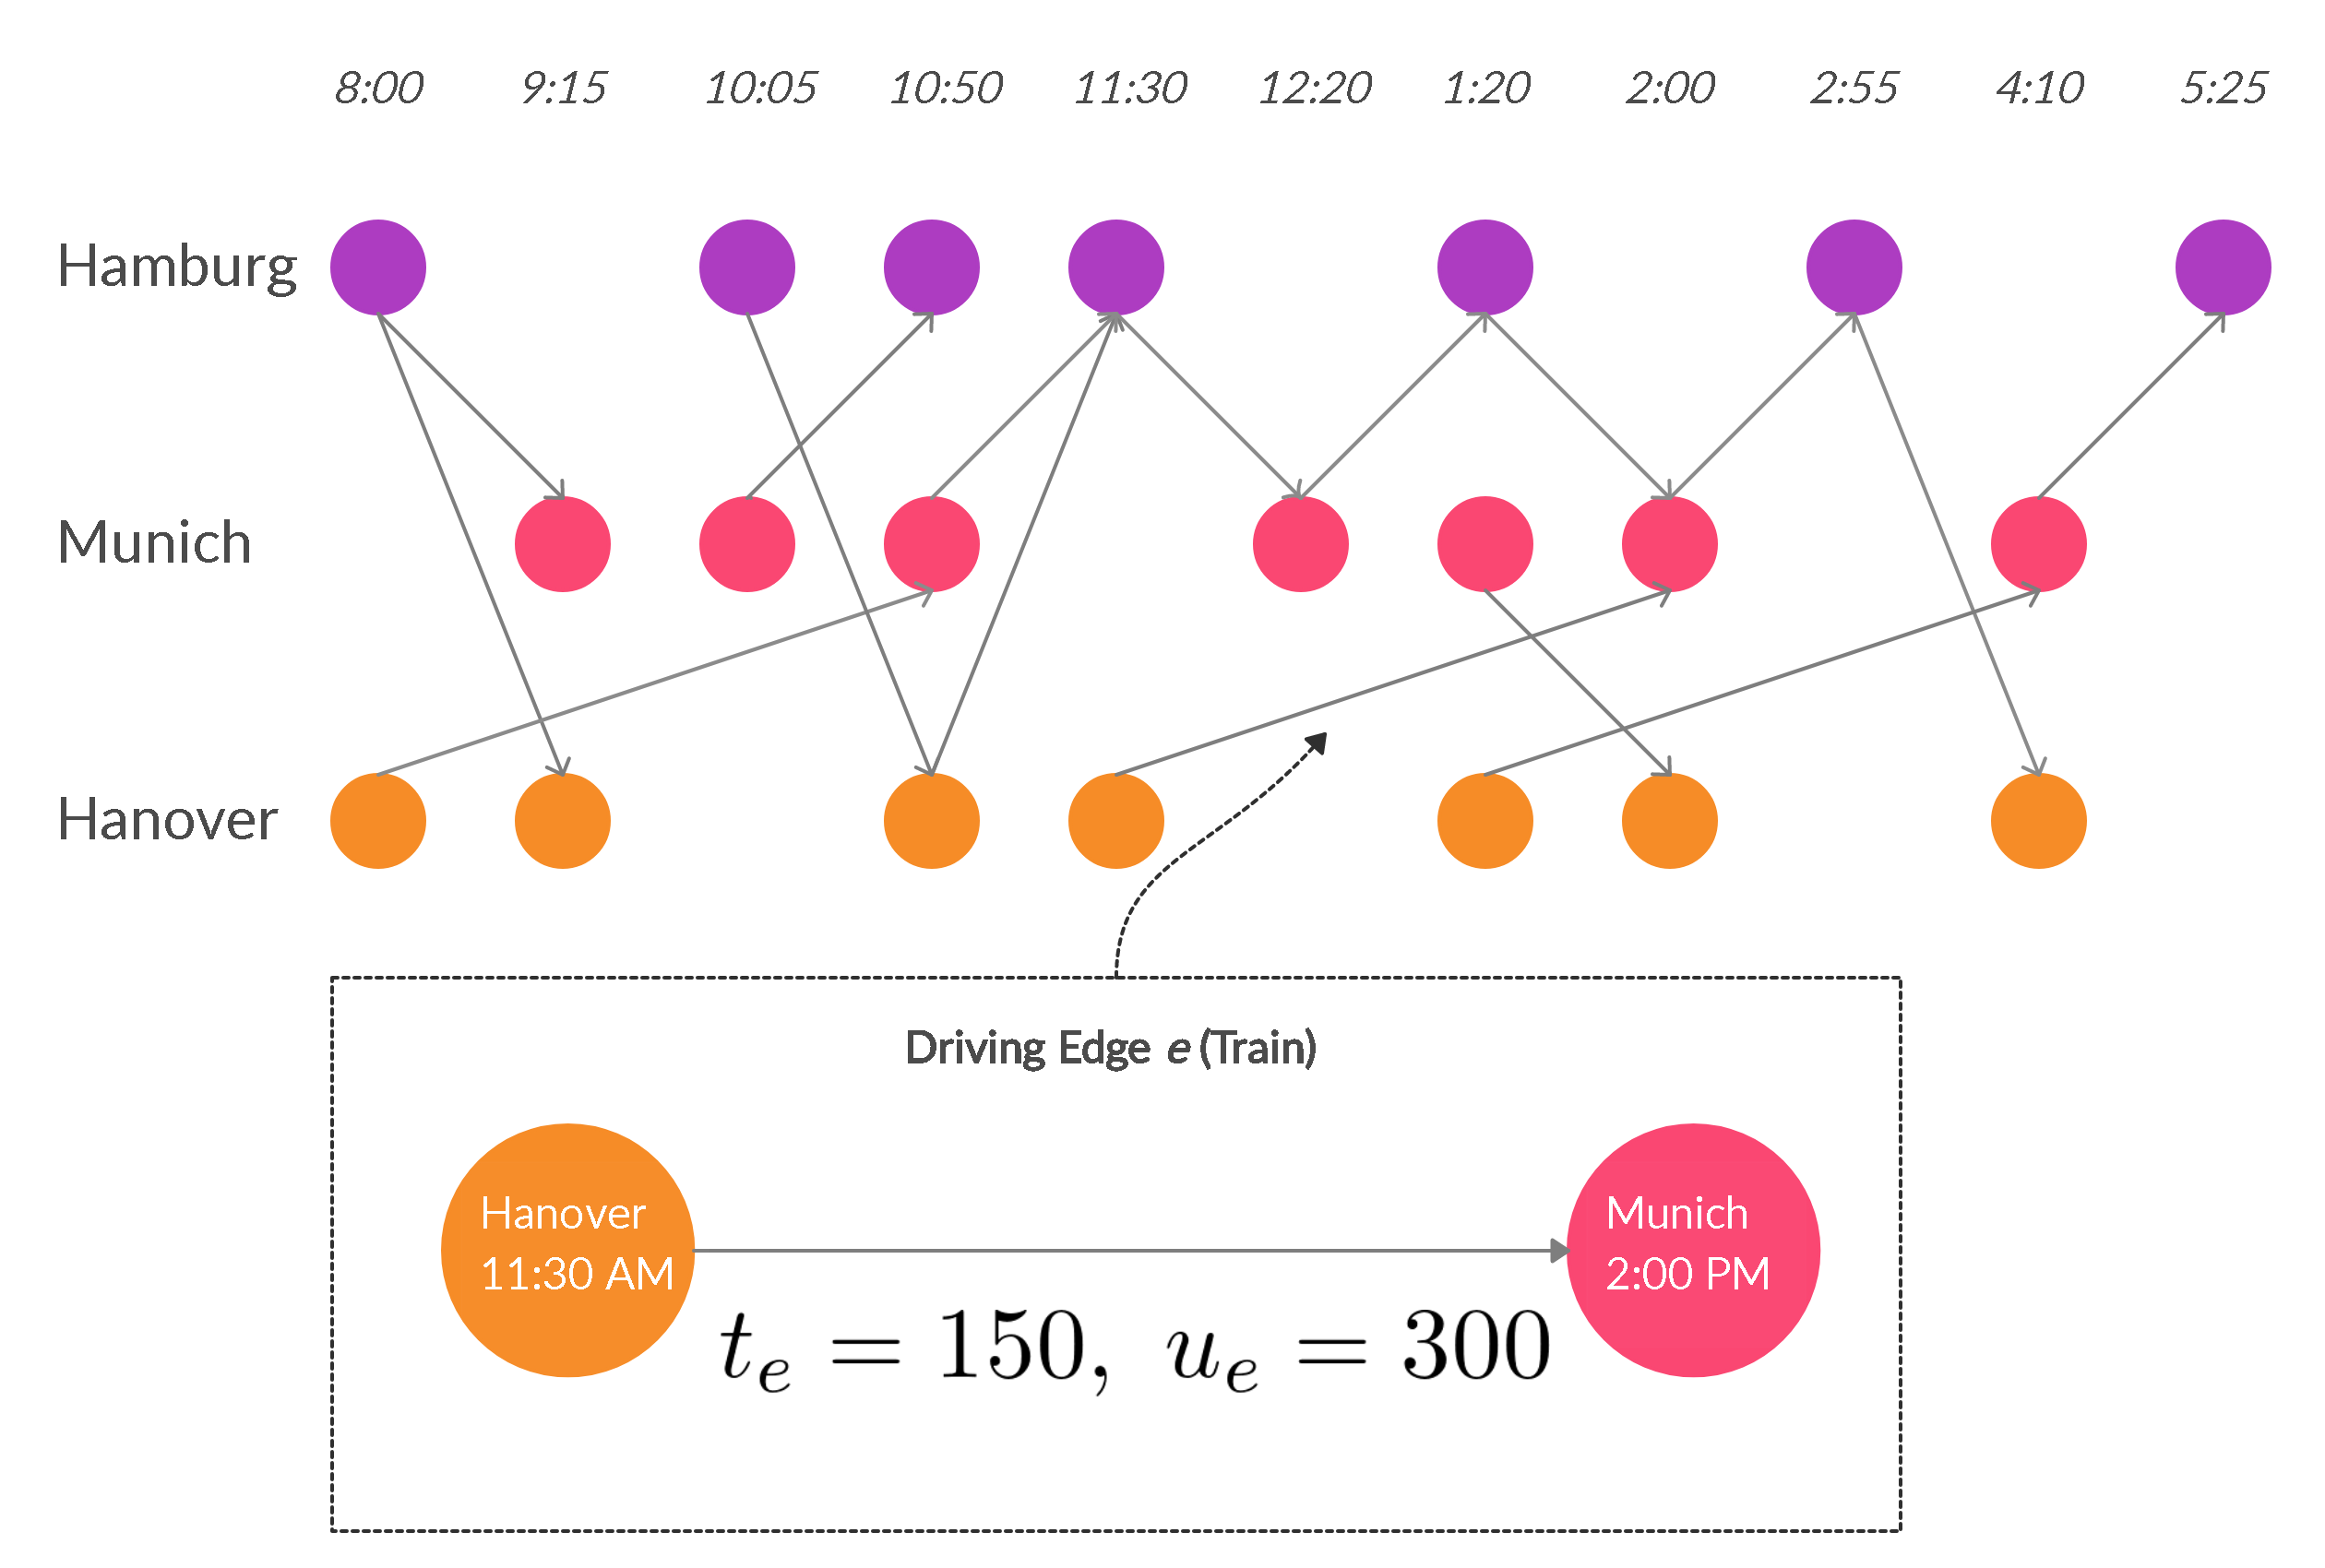
\includegraphics[scale=0.12]{Driving_Edges.jpg}
\end{figure}
\end{frame}

\begin{frame}{Network Representation: Waiting Edges}
\begin{figure}
    \centering
    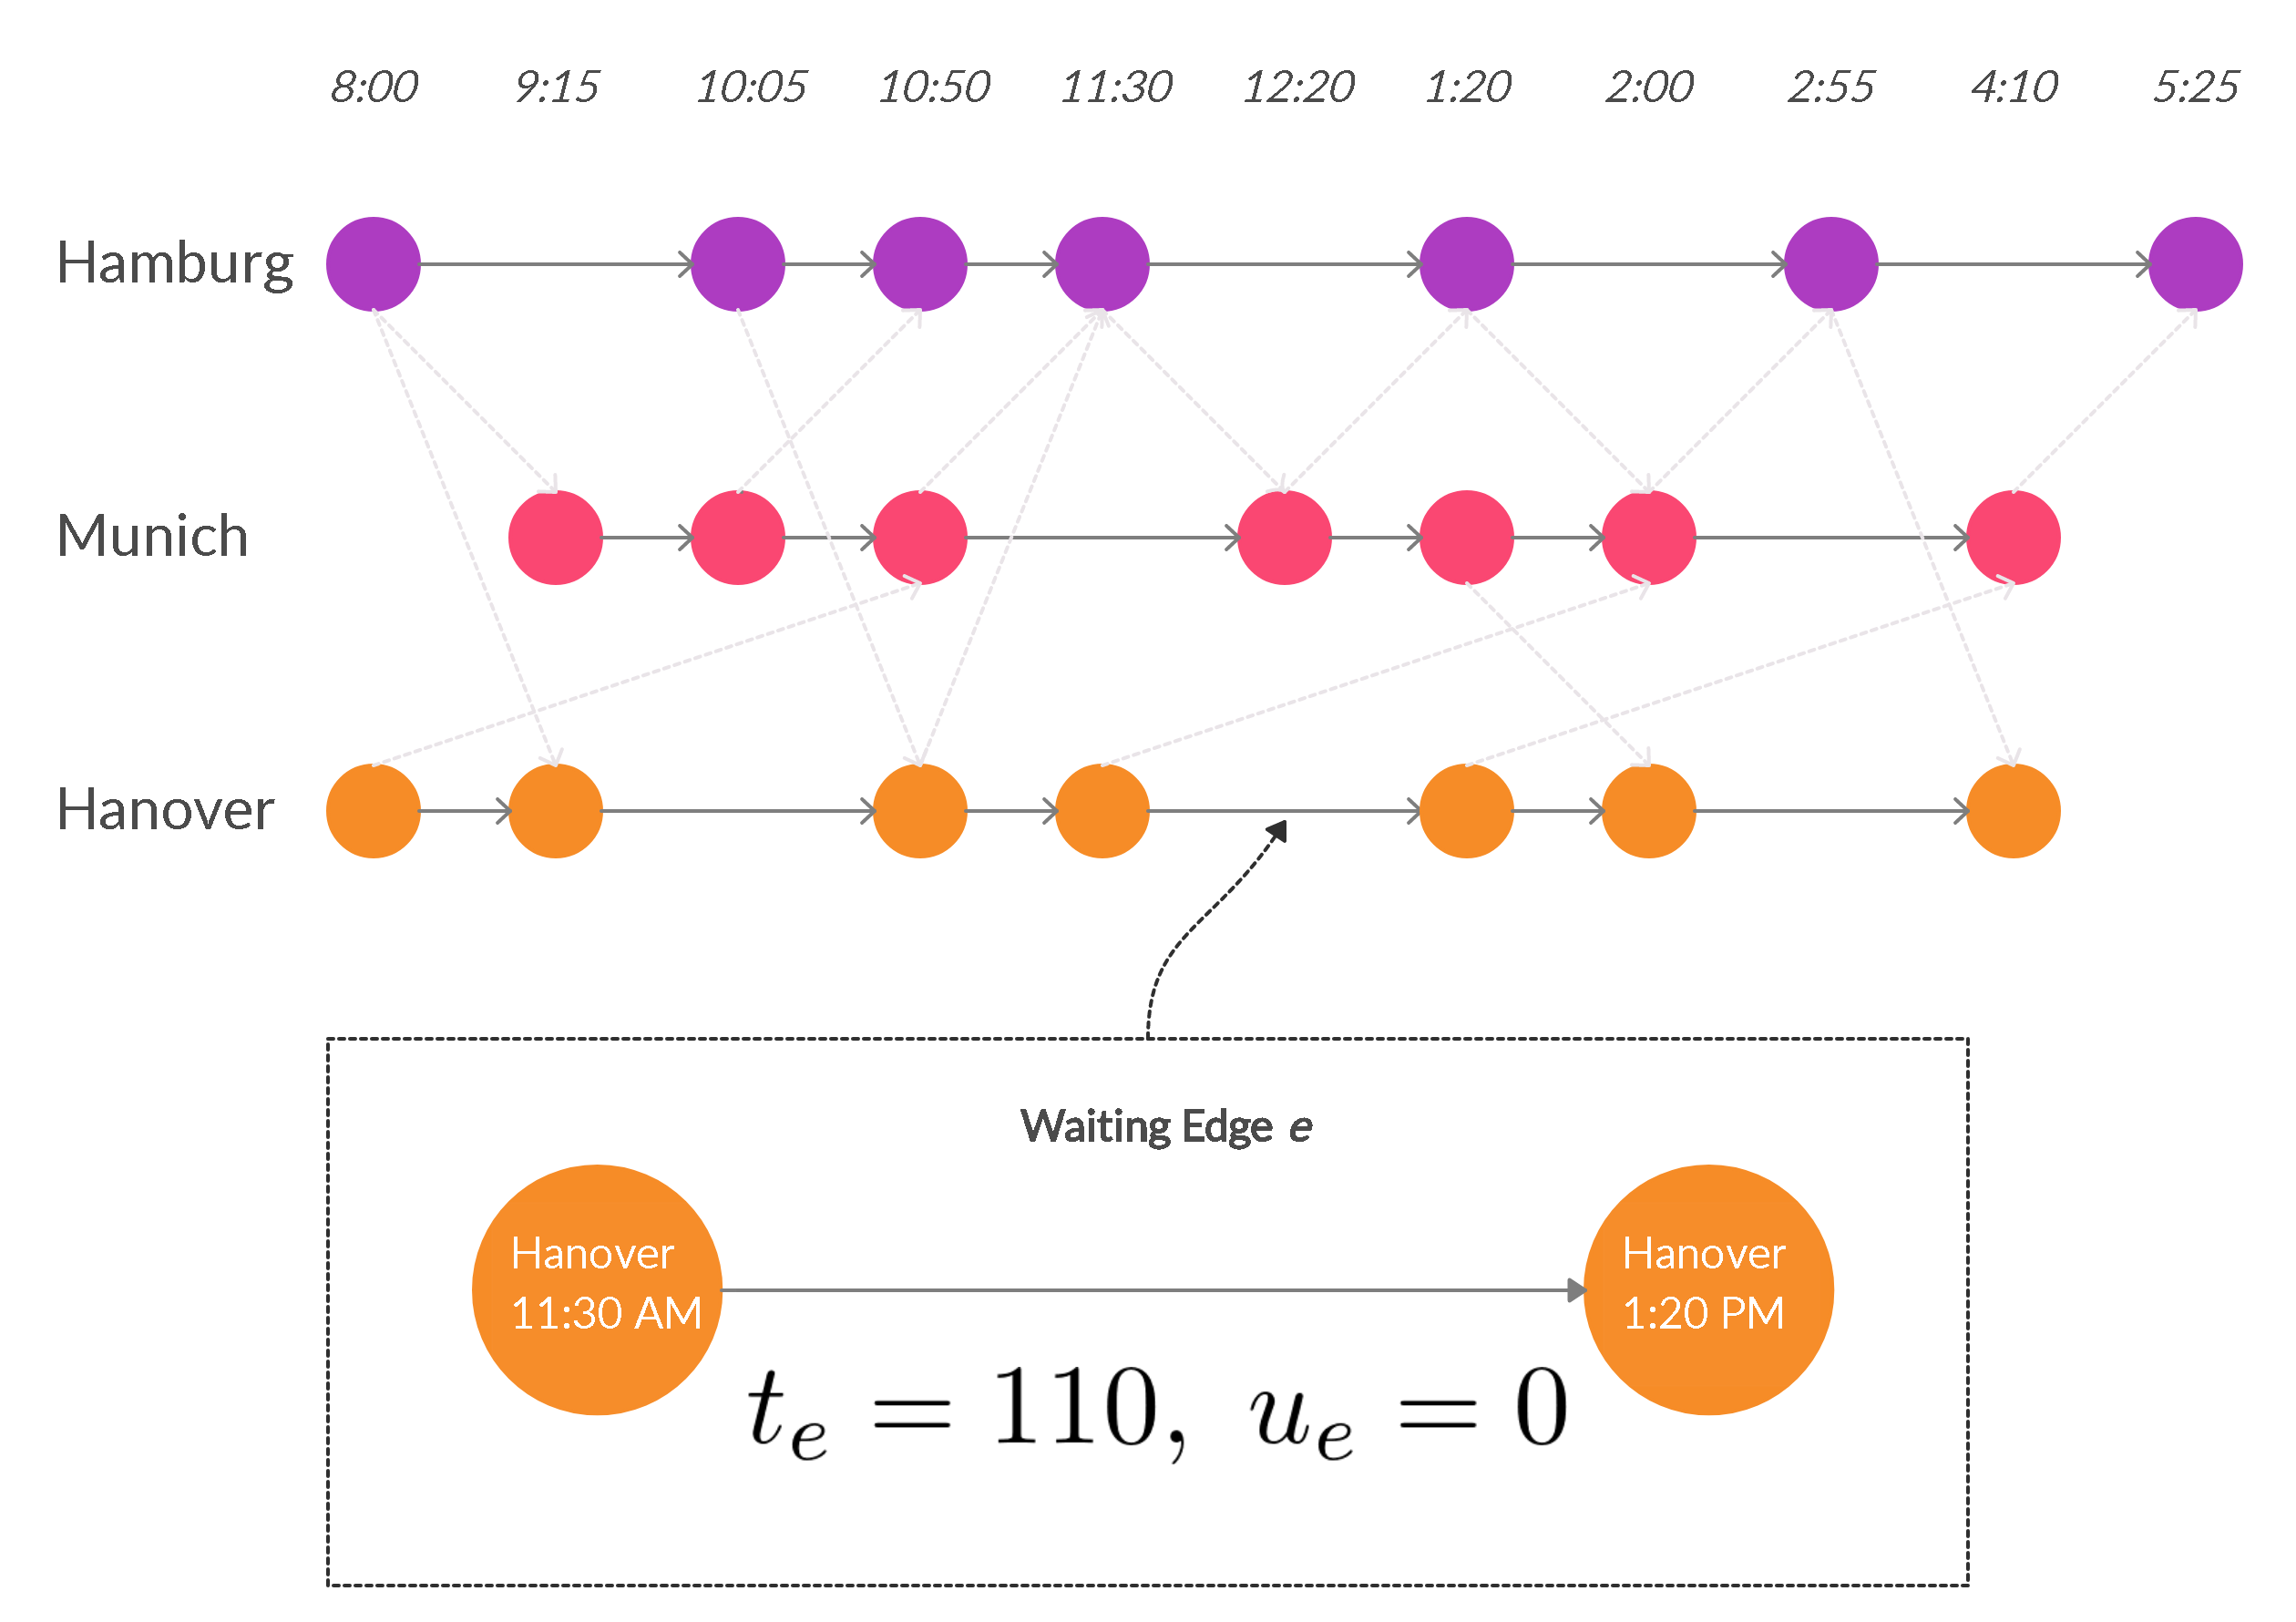
\includegraphics[scale=0.12]{Waiting_Edges.jpg}
\end{figure}
\end{frame}


\begin{frame}{Network Representation: Source and Sink}
\begin{figure}
    \centering
    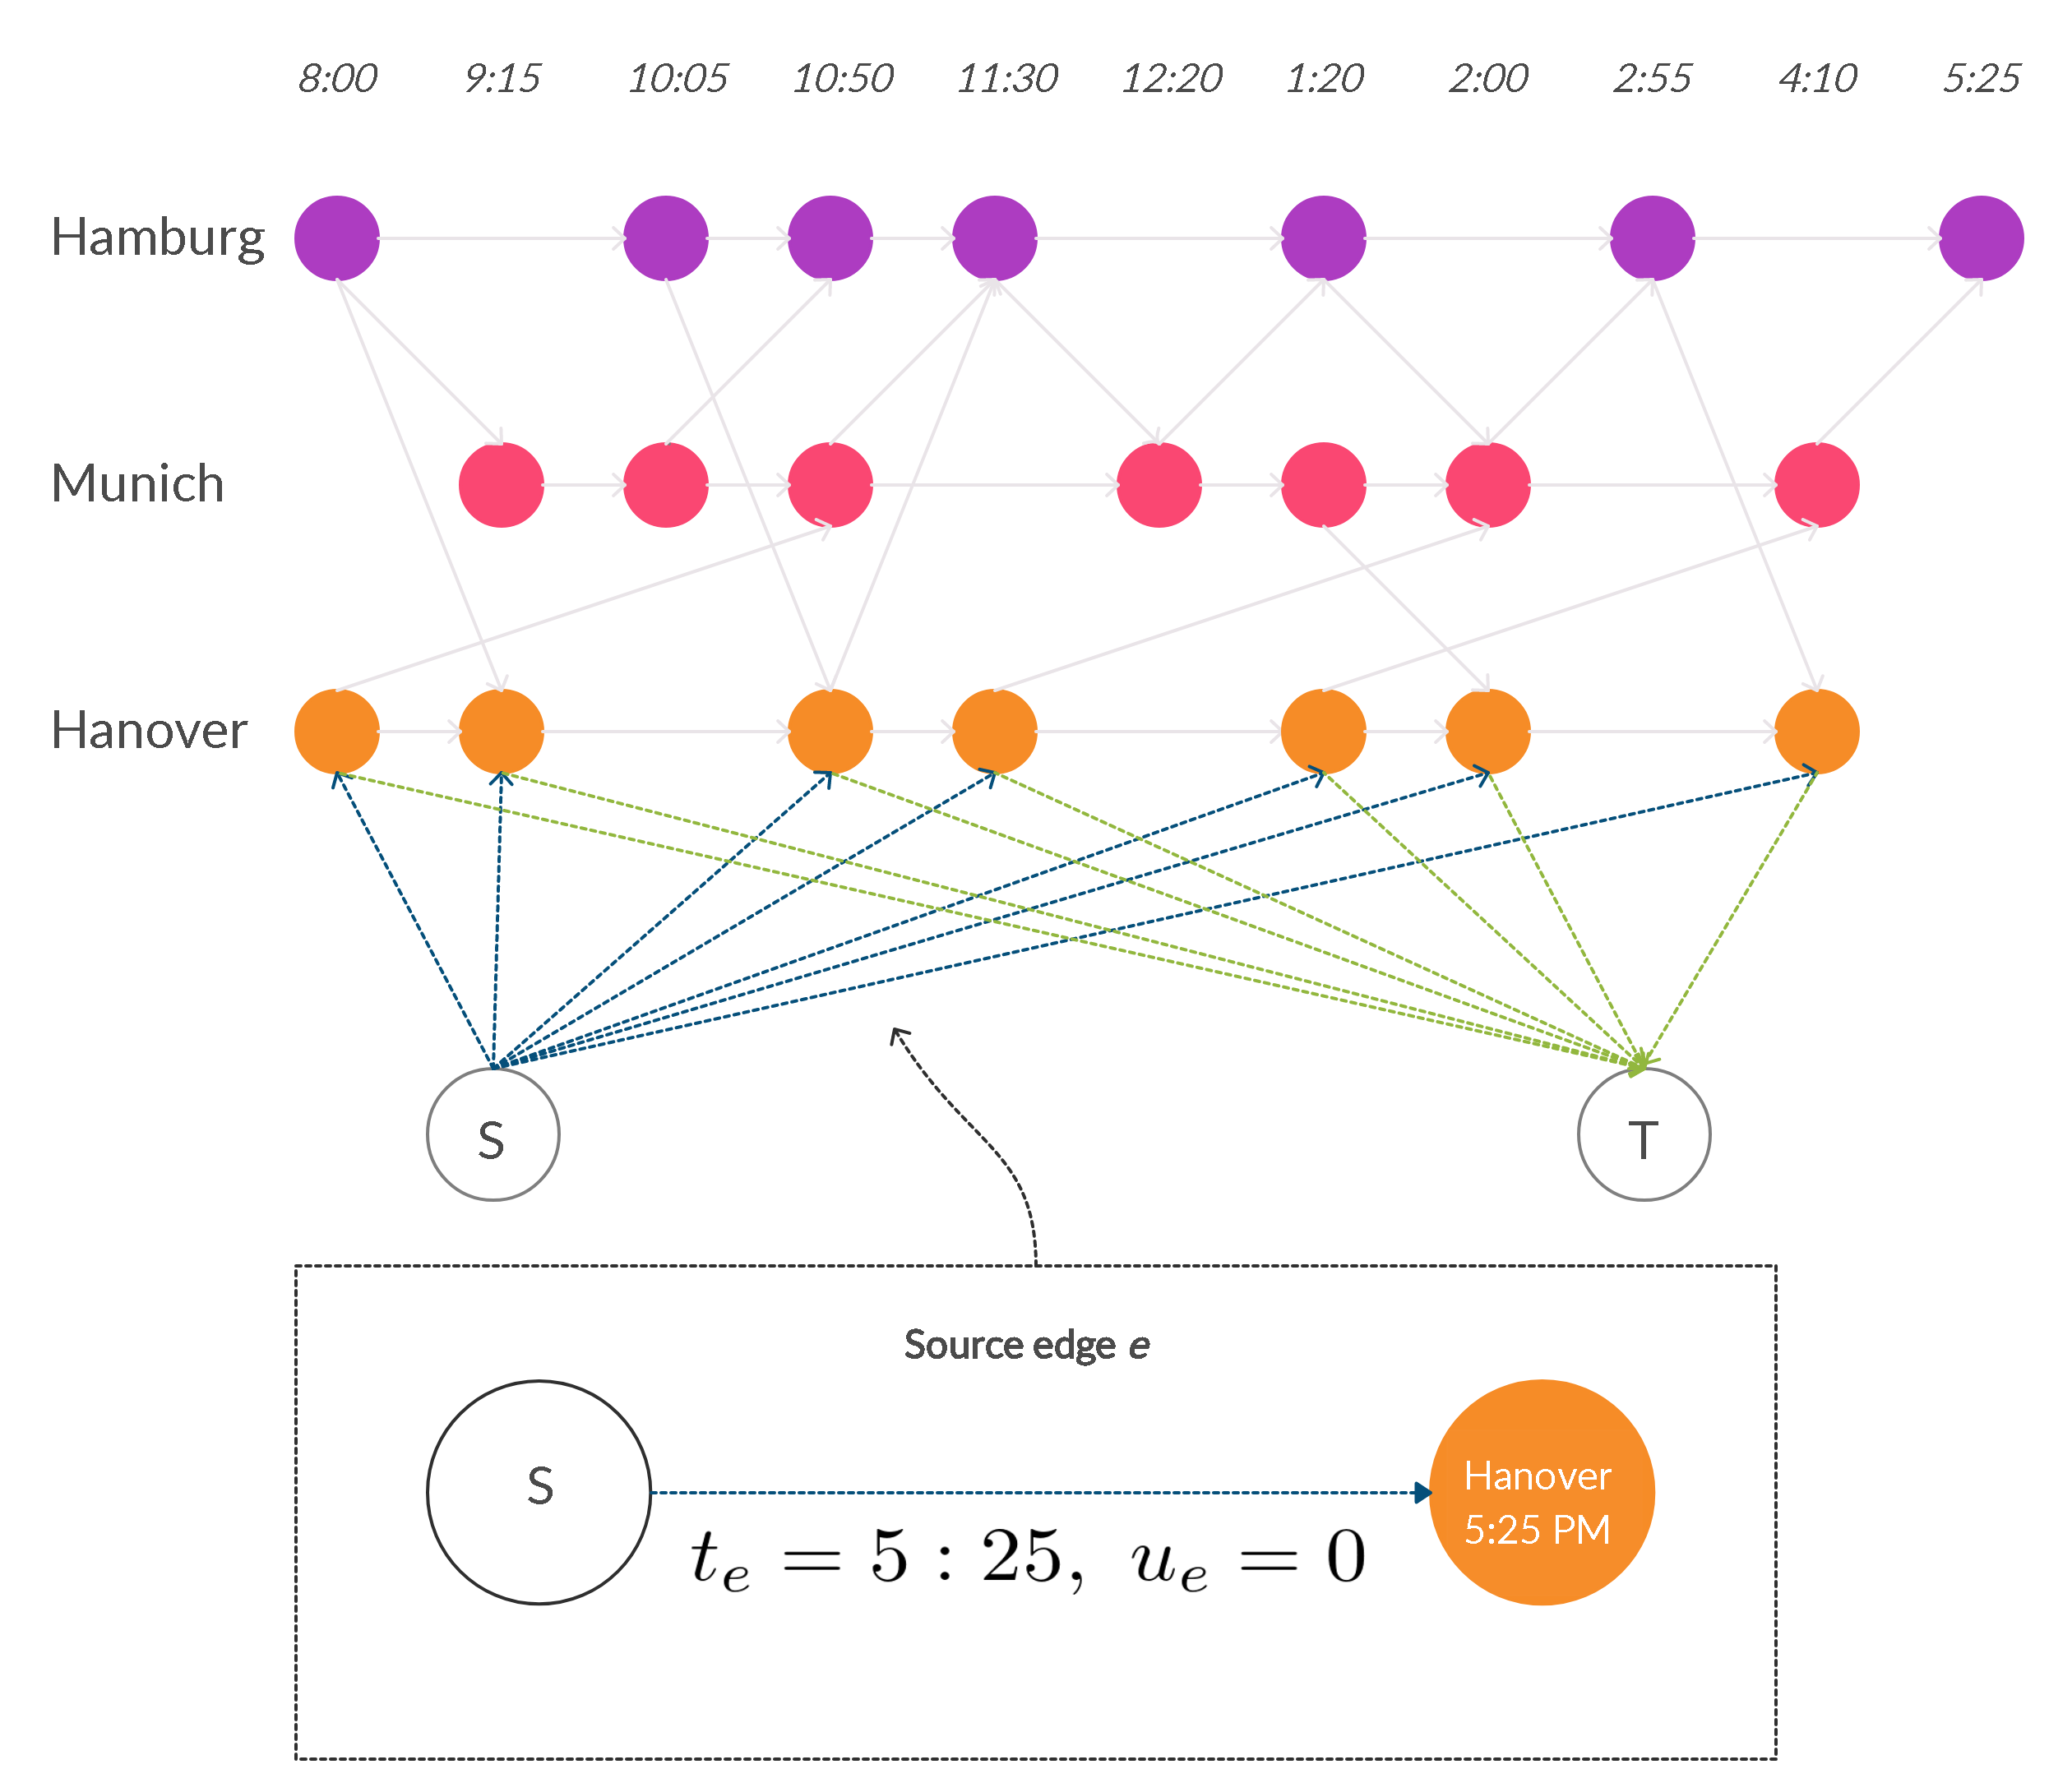
\includegraphics[scale=0.10]{Source_Sink_Edges.jpg}
\end{figure}
\end{frame}

\begin{frame}{Network Representation: Passenger Type}
\begin{figure}
    \centering
    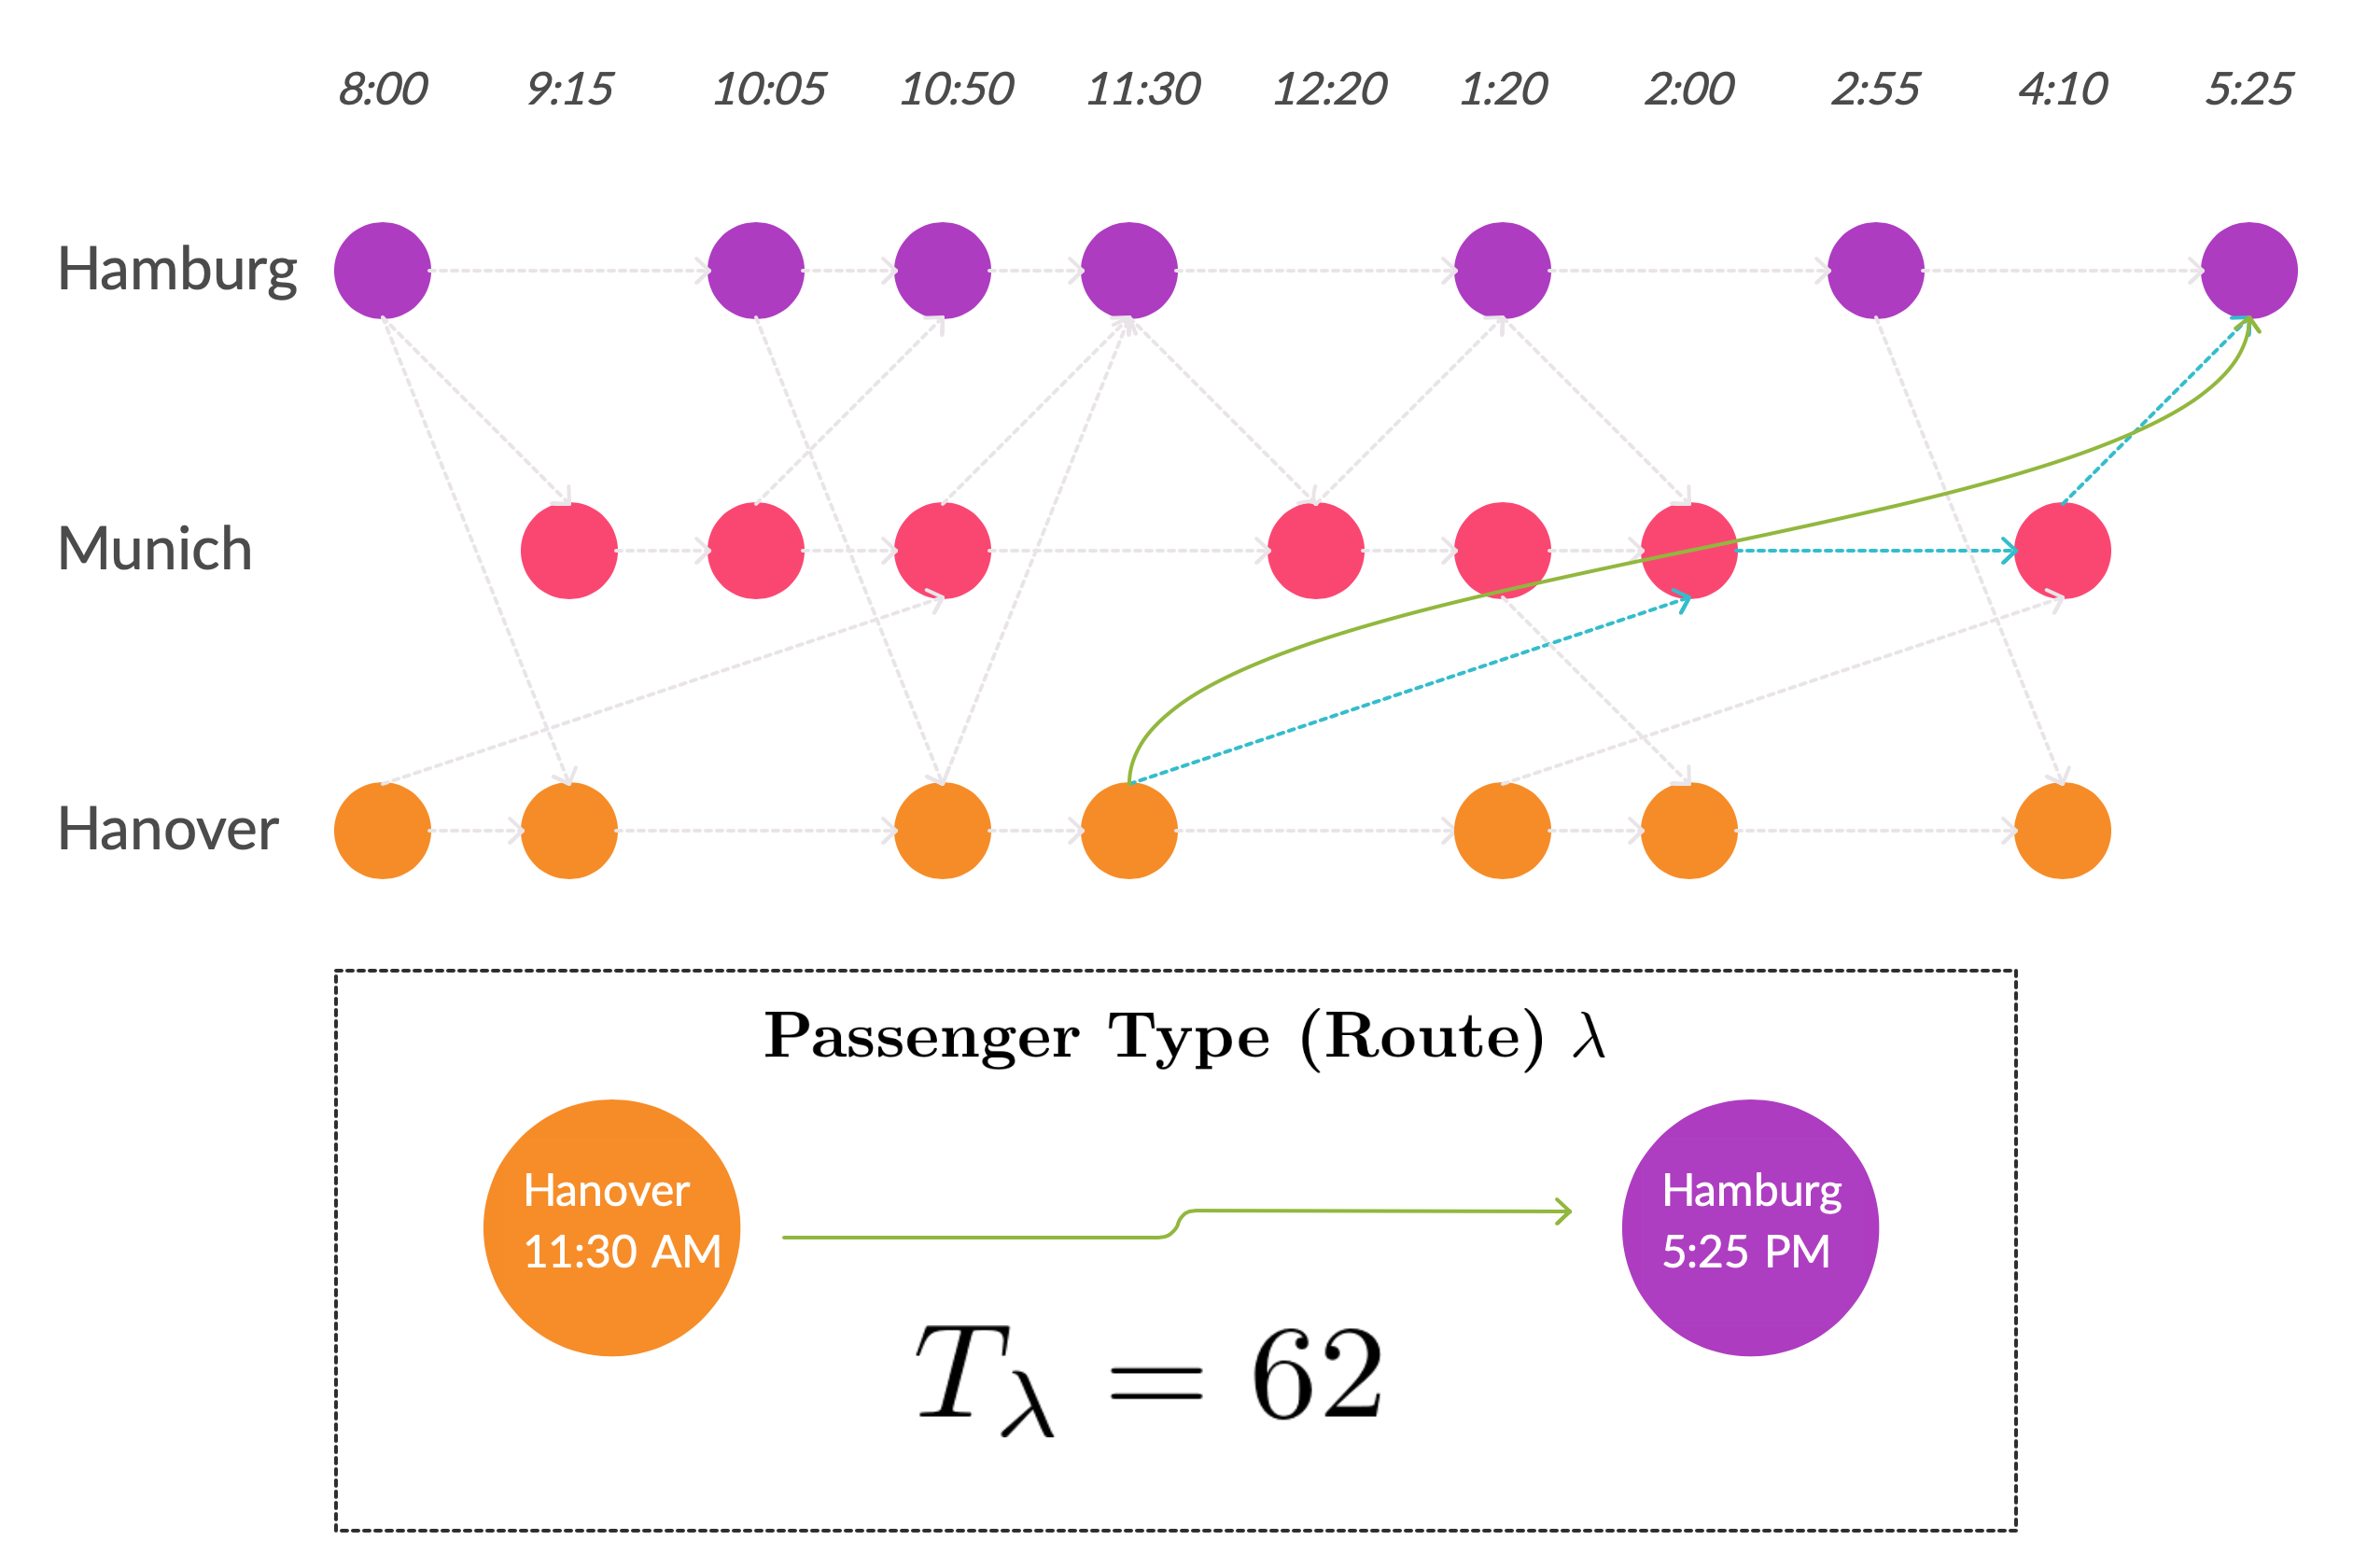
\includegraphics[scale=0.13]{Passenger_Path_Example.jpg}
\end{figure}
\end{frame}


\begin{frame}{Network Representation: Patrol}
\begin{figure}
    \centering
    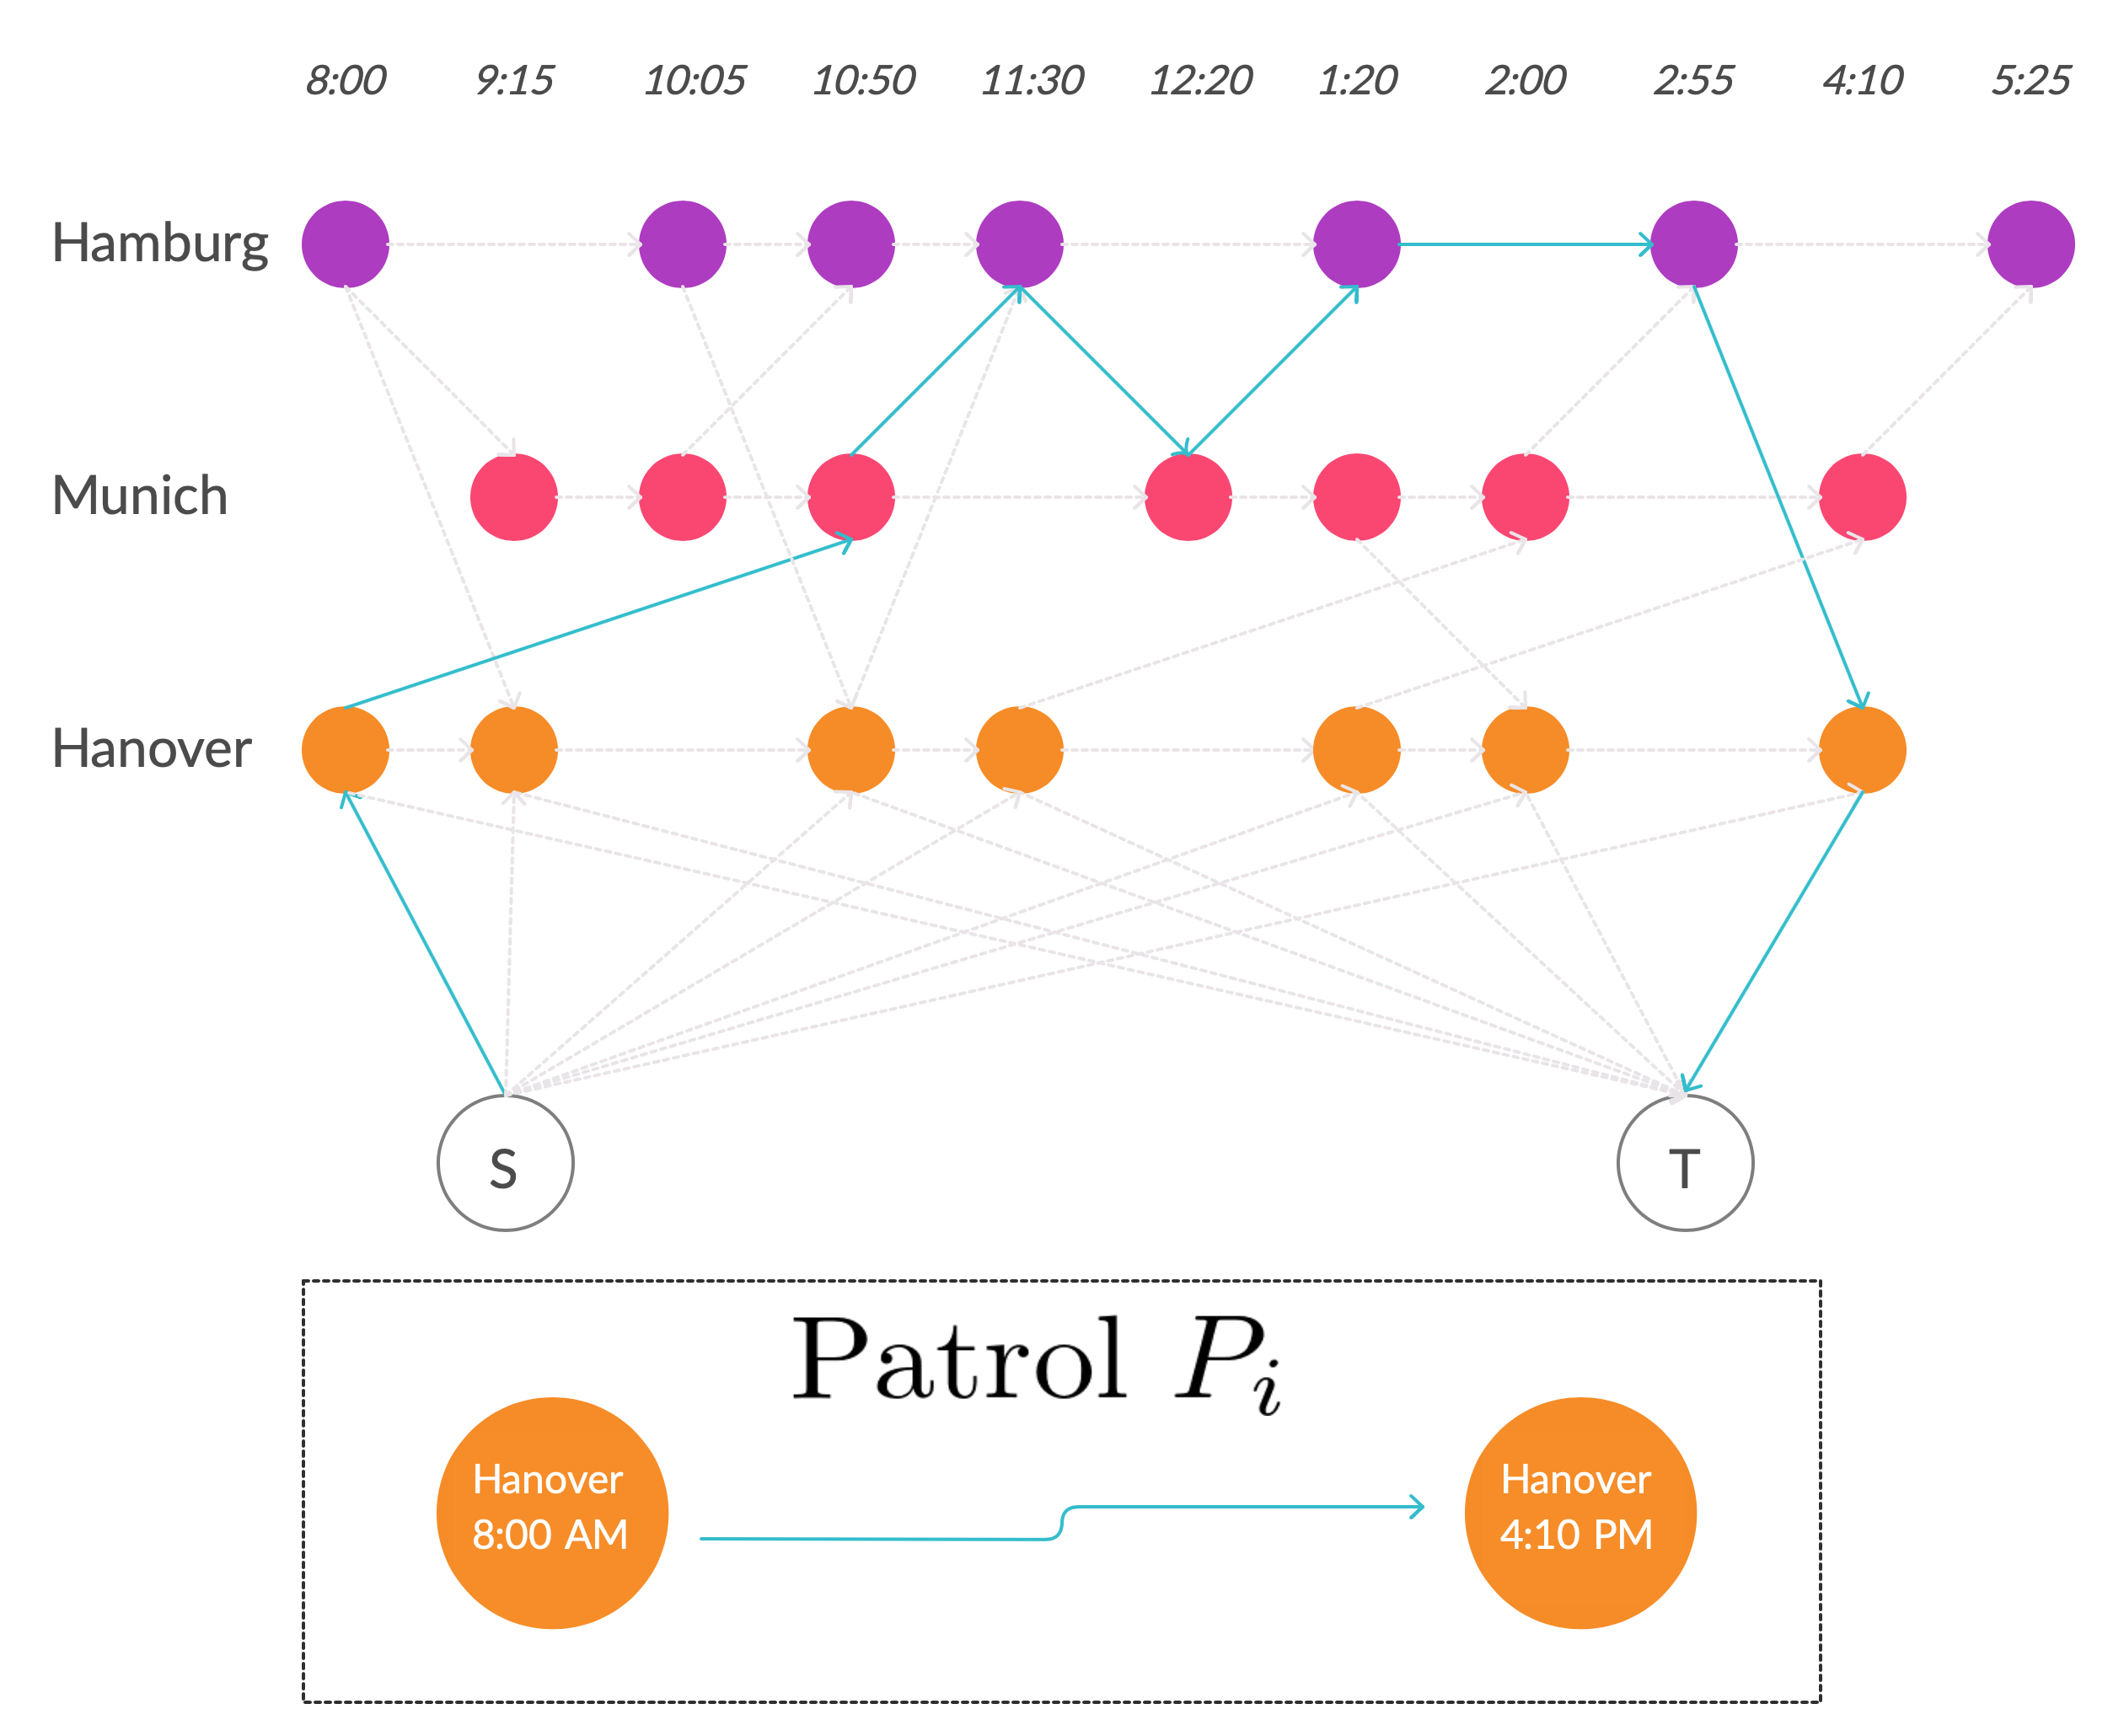
\includegraphics[scale=0.10]{Inspector_Path_Patrol.jpg}
\end{figure}
\end{frame}

\begin{frame}{Complexity Analysis}
    \textbf{Classification}: constrained shortest path problem.
   According to the appendices of \cite{Garey:1990:CIG:574848}, our problem is most similar to
   \begin{itemize}
        \item \textbf{Path Constrained Network Flow} [ND34]
        \begin{itemize}
            \item NP-Complete
        \end{itemize}
      
        \item \textbf{Vertex Covering (or restated arc Covering)} [GT1]
        \begin{itemize}
            \item Vertex covering is an NP-Complete problem
            \item arc covering can be solved in polynomial time using graph matching.
        \end{itemize}
        \item \textbf{Minimum Covering} [SP5]
        \begin{itemize}
            \item NP-Complete, but can become solvable in polynomial time under a specific assumption. 
        \end{itemize}
    \end{itemize}
    %Further work: reduce our problem into one of these to determine complexity.
    
\end{frame}

\begin{frame}{Patrol Strategies}
\begin{figure}
    \centering
    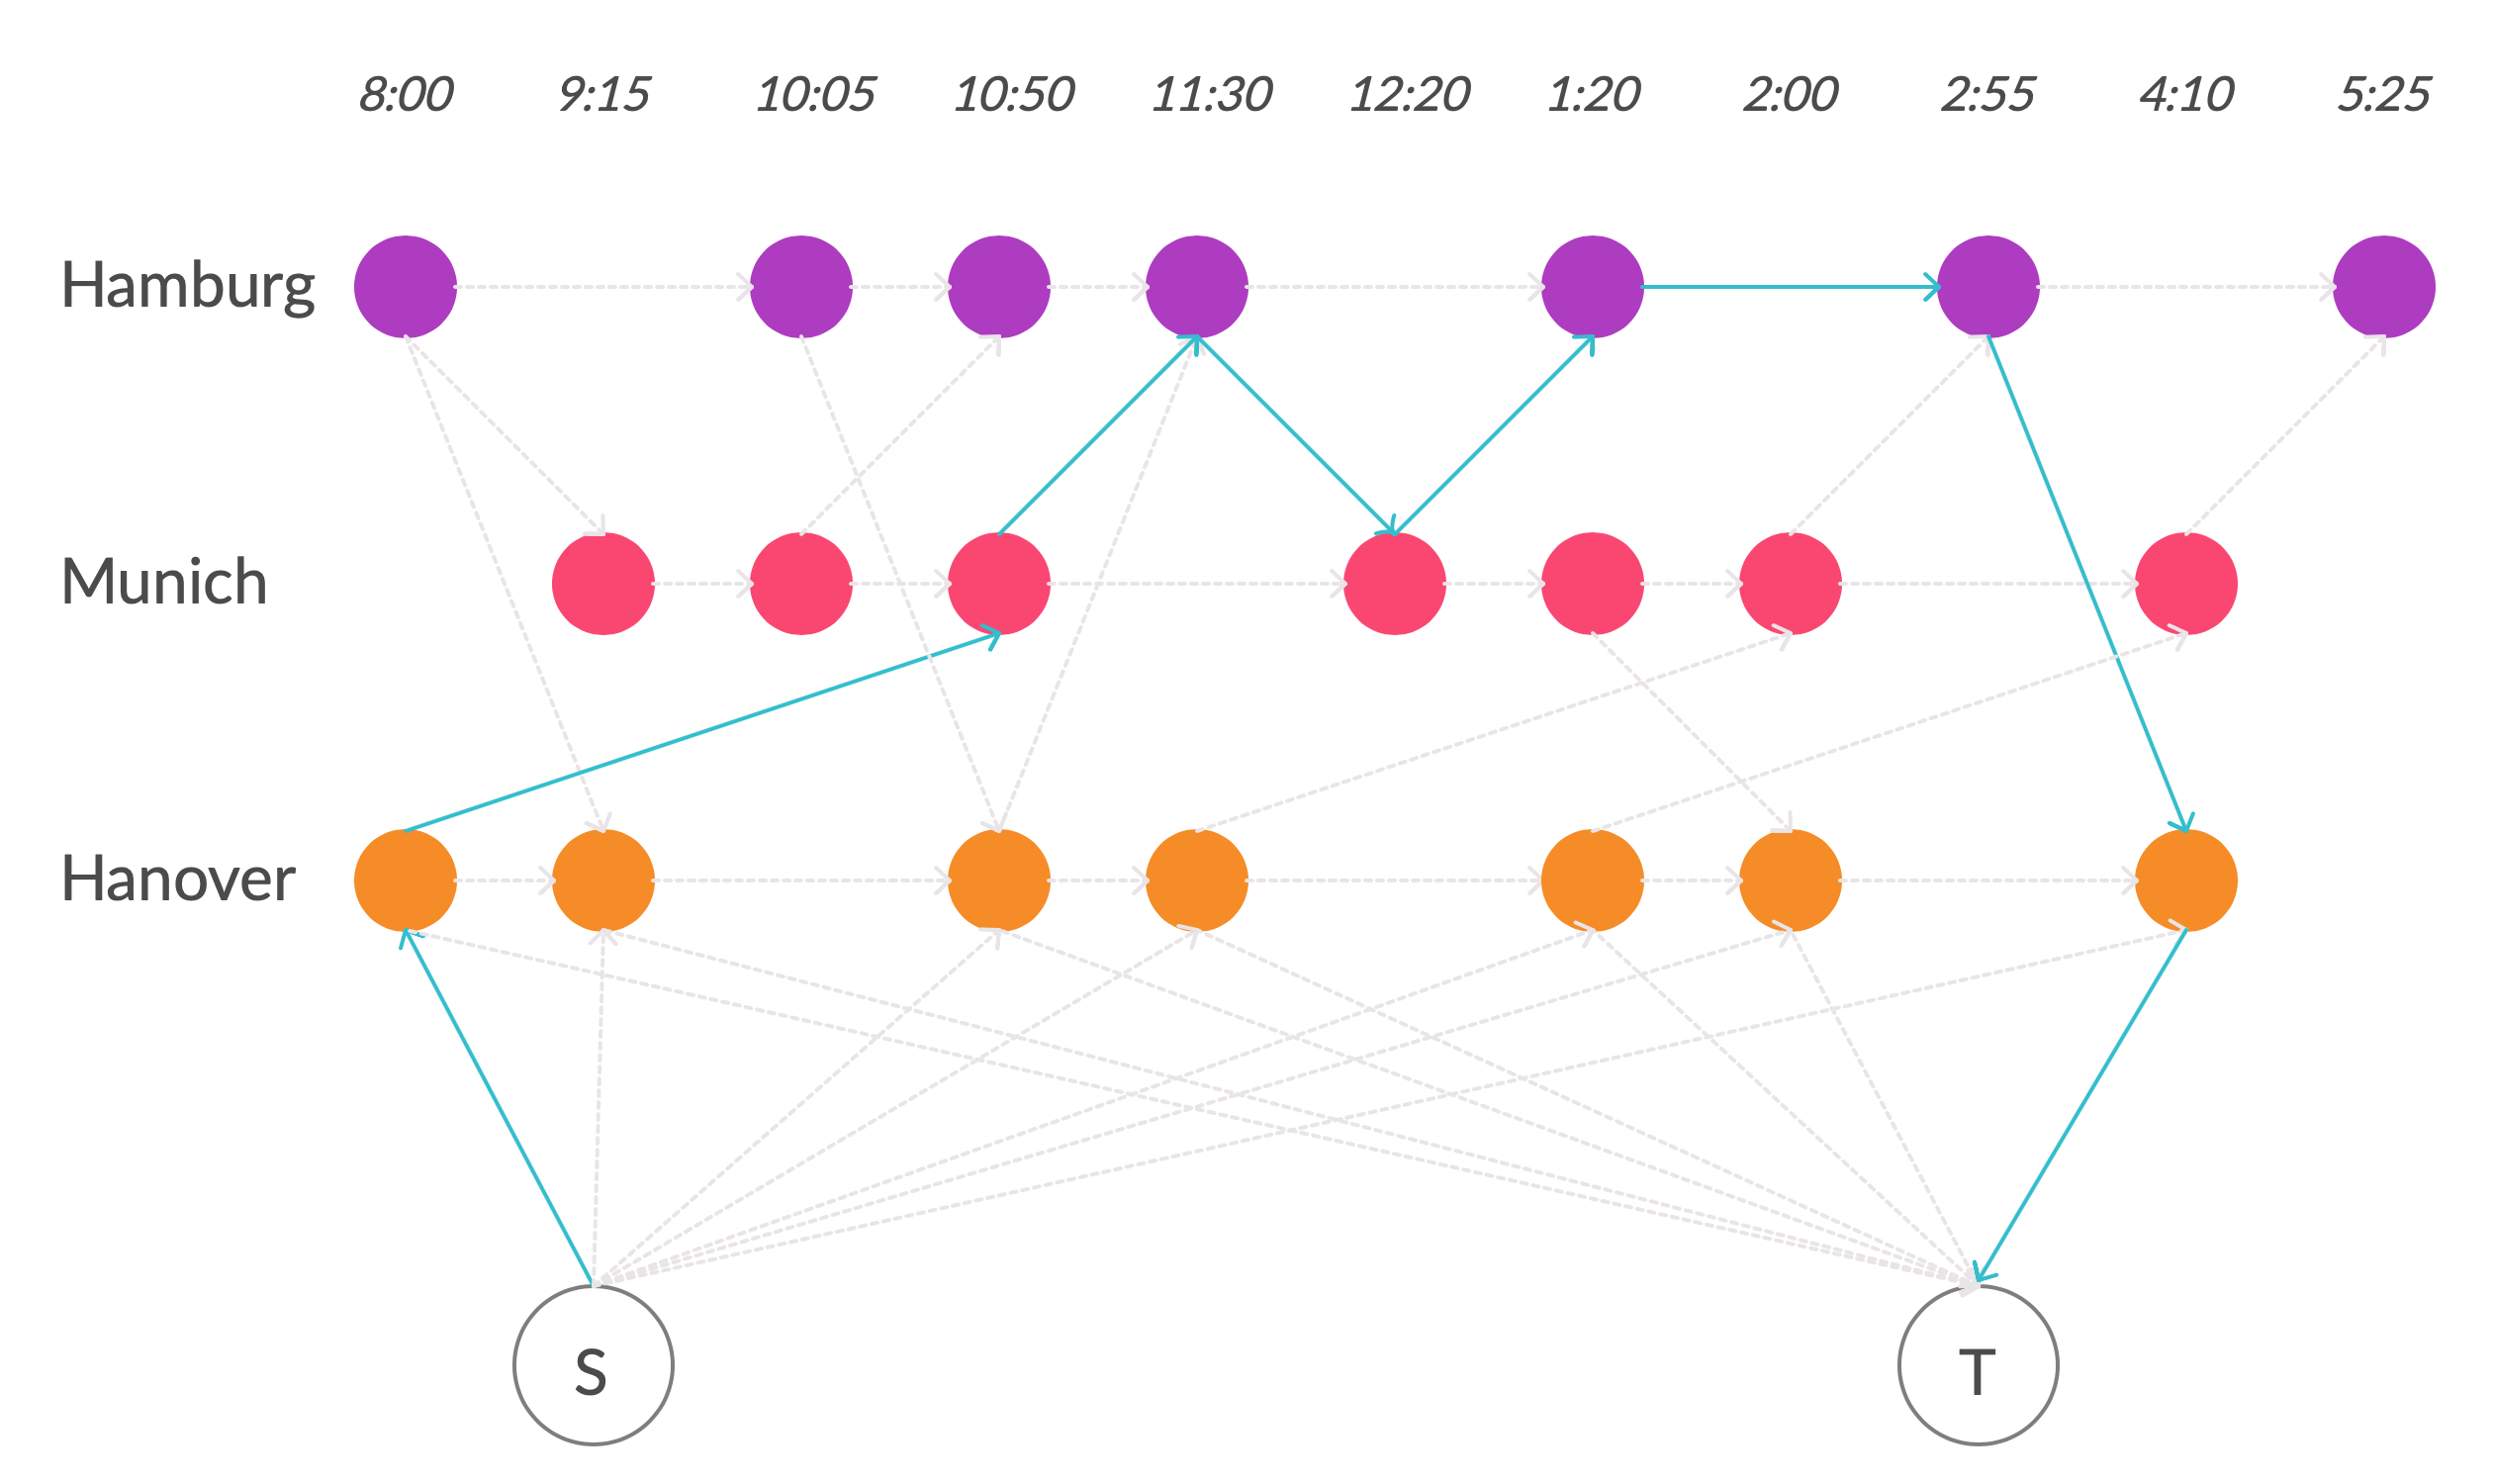
\includegraphics[scale=.09]{Inspector_Patrol_Binary.jpg}
\end{figure}
\begin{itemize}
    \item For the $i^{th}$ inspector, define \textbf{binary variables} $x_e^{(i)}$ for all edges $e$ in our graph.
    \item  If the inspector takes the train $e$, we set $x_e^{(i)} = 1$ and $0$ otherwise.
    \item A \textbf{patrol} $P_i$ can then be characterised by $\{x_e^{(i)}| x_e^{(i)} = 1 \}$ 
\end{itemize}
\end{frame}

%\subsection{Probability of Passenger Inspection}

\begin{frame}{Our Model: A Simple Look}
    \textbf{Our objective:}
\begin{align*}
    \max_x\quad \{\#\text{passengers inspected}\}
\end{align*}
\textbf{subject to:}
\begin{itemize}
    \item minimisation constraint
    \item time-flow constraint
    \item the flow-conservation (or mass-balance) constraint
    \item source constraint
    \item maximum number of inspectors allowed to work
\end{itemize}
\end{frame}


\begin{frame}{Source Constraint}
\begin{tcolorbox}[colback=yellow!5!white,colframe=yellow!75!black, title=Intuition]
If an inspector works, that inspector can only leave a source once.
\end{tcolorbox} 
\vspace{5mm}
\begin{tcolorbox}[colback=blue!5!white,colframe=blue!75!black]
\begin{align*}
        \sum_{e\in\delta^+(S_k)}x_e^{(k)} \le 1, \qquad \forall k\in K
\end{align*}
\end{tcolorbox}
\end{frame}

\begin{frame}{Flow Conservation Constraint}
 \begin{tcolorbox}[colback=yellow!5!white,colframe=yellow!75!black, title=Intuition]
  If an inspector arrives at a station, that inspector must leave that station.
\end{tcolorbox} 
\vspace{5mm}

\begin{tcolorbox}[colback=blue!5!white,colframe=blue!75!black]
\begin{align*}
        \sum_{e\in\delta^+(B)}x_e^{(k)} - \sum_{e\in\delta^-(B)}x_e^{(k)} = 0, \qquad \forall B\in N,\quad \forall k\in K
\end{align*}
\end{tcolorbox}
\end{frame}


% Nate
\begin{frame}{Time Flow Constraint}
\begin{tcolorbox}[colback=yellow!5!white,colframe=yellow!75!black, title=Intuition]
   For each inspector, the difference between the time of arrival and departure from a base station is less than the maximum allotted time to work.
\end{tcolorbox} 
\vspace{5mm}

\begin{tcolorbox}[colback=blue!5!white,colframe=blue!75!black]
\begin{align*}
        \sum_{e\in\delta^-(T_k)}x_e^{(k)}\cdot t_e - \sum_{e\in\delta^+(S_k)}x_e^{(k)}\cdot t_e \le \theta_k,\qquad \forall k\in K
\end{align*}
\end{tcolorbox}
\end{frame}

\begin{frame}{Max Number of Inspectors constraint}

\begin{tcolorbox}[colback=yellow!5!white,colframe=yellow!75!black, title=Intuition]
  The maximum number of inspectors allowed to work is $\kappa$.
\end{tcolorbox}
\vspace{5mm}

\begin{tcolorbox}[colback=blue!5!white,colframe=blue!75!black]
\begin{align*}
        \sum_{k\in K} \sum_{e\in\delta^+(S_k)}x_e^{(k)}\le \kappa,\qquad \ \kappa \in \mathbb{N}
\end{align*}
\end{tcolorbox}
\end{frame}

% Ruby
\begin{frame}{Probability of Passenger Inspection}
    \begin{itemize}
        \item We classify passengers according to their path (time of departure, origin, destination). 
        \item A passenger of type $\lambda$ is a passenger who is travelling path $\lambda$ \pause
        
        \item The \textbf{``probability''} that a passenger of type $\lambda$ is inspected is \citep{jiang_yin_johnson_tambe_kiekintveld_leyton-brown_sandholm_2012}
    \begin{align*}
       \min\bigg\{1,\sum_{i=1}^K\sum_{e\in P_i\cap\lambda} f_e\bigg\}
    \end{align*}
    where:
    \begin{itemize}
        \item $f_e$ -- \textit{inspector effectiveness} value assigned to edge $e$
        \item $P_i$ -- the patrol strategy for the $i^{th}$ inspector
        \item $\lambda$ -- a particular path taken by a passenger
        %\item $\Pi_\lambda$ -- probability that a %passenger of type $\lambda$ is inspected
    \end{itemize}
    \end{itemize}
\end{frame}

% Nate
\begin{frame}{Objective Function Formulation}
   \textbf{Maximise} the number of inspected passengers of all types:
    \begin{align*}
        \max_{\textbf{x}} \sum_{\lambda\in \Lambda}\underbrace{T_{\lambda}\cdot \min\bigg\{1,\sum_{e\in\lambda}f_e\bigg(
            \sum_{i=1}^K x_{e}^{(i)}
        \bigg)\bigg\}}_{\text{Expected \#passengers of type $\lambda$ inspected}}
    \end{align*}
    \pause
    We re-write this as a LP problem: \pause
    \begin{align*}
         \uncover<+->{&\quad \quad \quad \quad 
        \max_{\textbf{x}} \sum_{\lambda \in \Lambda} T_\lambda \cdot \Pi_{\lambda}(x)\\}
         \uncover<+->{& \text{subject to}\\
        &\quad \quad \quad \quad 
        \Pi_\lambda(x) \le 1\\
        & \quad \quad \quad \quad
        \Pi_\lambda(x) \le \sum_{e\in\lambda}f_e\bigg(
            \sum_{i=1}^K x_{e}^{(i)}
        \bigg)}
    \end{align*}
    
    % Issue: how do we determine the number of passengers of each type, $T_\lambda$?

\end{frame}


%\section{Issues}
%\begin{frame}{Issues}
    %\begin{itemize}
        %\item Due to the massive complexity of the %problem we face the following questions.
            %\begin{itemize}
                %\item How do we pick the optimal %subset of our resources (523 %inspectors) to maximise the span %of the graph?
                %\item Which bases are optimal for %spanning? 
                %\item How many inspectors are %needed?
            %\end{itemize}
        %\item Passenger Route Estimation
            %\begin{itemize}
                %\item sdf
            %\end{itemize}
    %\end{itemize}
%\end{frame}

%\begin{frame}{Current Ideas}
    %Implementing a \textbf{local search}. Issues %arising with this: reducing the dimensionality %of the problem and fixing specific solutions. %how do we go about doing this? Comparing %theoretical models.
        %\begin{itemize}
            %\item Solving the problem for 1 %inspector is quick (even for 2, or 3 %is reasonable).
            %\item Suppose we introduce 20 %inspectors and fix the path for 19 %inspectors. We expect the same %solutions. Experiments say this takes %longer.
            
            %\item We may compromise the optimality %of solutions for just ``good" %solutions.
        %\end{itemize}
%\end{frame}
\begin{frame}{Passenger Classification Estimation (OD Matrix)}
\begin{itemize}
    \item We do not actually have this information, we only have passenger counts
    \item Estimate using an \textbf{information minimising}/\textbf{entropy maximising} method by \cite{van_zuylen_willumsen_2002} which requires no prior knowledge.\pause
\end{itemize}

\begin{tcolorbox}[colback=blue!5!white,colframe=blue!75!black,title=Input]
 Train passenger volumes, all possible passenger route
\end{tcolorbox}

%output box
\begin{tcolorbox}[colback=yellow!5!white,colframe=yellow!75!black,title=Output]
 Entries $(i,j)=:\lambda$ of a matrix representing the 
 estimated number of passengers of type $\lambda$.
\end{tcolorbox}

\end{frame}


\begin{frame}
  \vfill
  \centering
  \begin{beamercolorbox}[sep=8pt,center,shadow=true,rounded=true]{title}
    \usebeamerfont{title} Implementation and Experiments \par%
  \end{beamercolorbox}
  \vfill
  \end{frame}
  
\section{Implementation and Experiments}
\begin{frame}{Experiments\footnote{On MacBook Pro ver. 2017, 3.3 GHz Intel Core i5, 8GB RAM.}}
\begin{itemize}
    \item Implement using Gurobi API for Python.
    \item Produce inspection schedule for the \textbf{ICE 401 Fleet} on \textbf{Monday}.
\item The graph has 3593
driving arcs and 4667 waiting arcs. 
\item 157 stations involved in the train schedule on Monday.
\item Take about 18.66 seconds to estimate the OD matrix.
\item Set the gap tolerance (called MIPGAP)  to 10\% and 5\%.
\item Record the \textbf{CPU/Wallclock time} taken by the programme.
\end{itemize}
 \end{frame}
 
 \begin{frame}{Example Solution}
     \begin{figure}
         \centering
         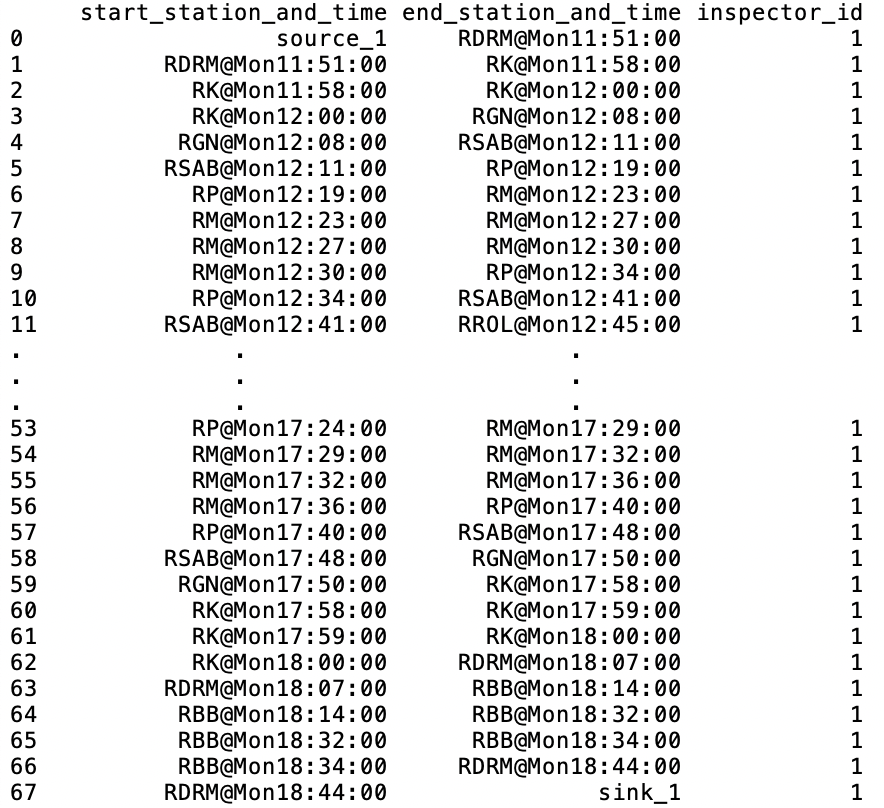
\includegraphics[scale=0.5]{example_sol.png}
         %\caption{Caption}
         %\label{fig:my_label}
     \end{figure}
 \end{frame}


  
\begin{frame}{Experiment Results (Data)}
\begin{table}[]
    \centering
    \begin{tabular}{|c|c|c|c|c|}
        \hline
        \multicolumn{2}{|c|}{\#\textbf{Inspectors}} & \multicolumn{2}{l|}{\textbf{CPU/Wallclock time (in seconds)}} \\ \cline{3-4} 
         \multicolumn{2}{|c|}{}  & \textbf{MIPGAP 5}\%           & \textbf{MIPGAP 10}\%           \\ \hline
        \multicolumn{2}{|l|}{1 (1 Depot)} & $< 1$                & $< 1$                   \\ \hline
        \multicolumn{2}{|l|}{2 (2 Depots)}  & $9$                 &  $4$           \\ \hline
        \multicolumn{2}{|l|}{4 (4 Depots)}  & $39$                 &  $24$           \\ \hline
        \multicolumn{2}{|l|}{6 (4 Depots)}  & $36$                 &  $30$           \\ \hline
        \multicolumn{2}{|l|}{10 (7 Depots)}  & $300$                 &  $104$           \\ \hline
        \multicolumn{2}{|l|}{15 (10 Depots)}  & $505$                 &  $160$           \\ \hline
        \multicolumn{2}{|l|}{30 (10 Depots)}  & $5617$                 &  $976$           \\ \hline
    \end{tabular}
    \caption{Empirical running time for different set of inspectors.}
    \label{tab:runtime-without-heuristic}
\end{table}
\end{frame}

\begin{frame}{Experiment Results (Plot)}
    \begin{figure}
        \centering
        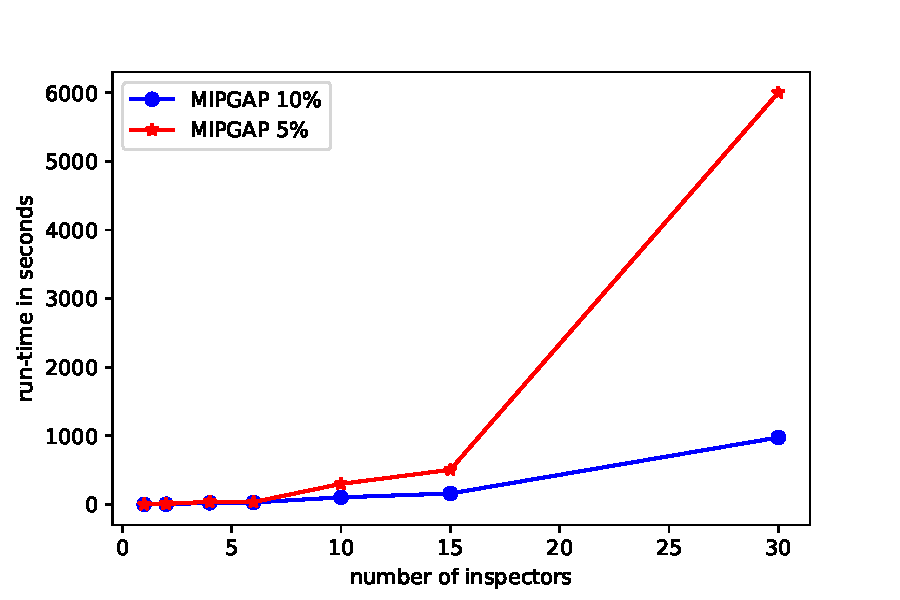
\includegraphics[scale=0.6]{runtime.pdf}
        \caption{Run time as number of inspectors grows for two different Gap tolerances.}
        \label{fig:my_label}
    \end{figure}
\end{frame}

\section{Heuristic Solver for Large-Scale Problem}

\begin{frame}{Developing Heuristic Solvers}
\begin{itemize}
    \item \textbf{Problem}: Running time seems to increase \textbf{exponentially} 
    w.r.t. the number of inspectors.
    \item \textbf{Proposed Solution}: Reduce the number of \textbf{undefined}
    variables currently in the model
    by ruling out others (i.e., set their values to zero). 
\end{itemize}

\begin{block}{Heuristic Solver for Large-Scale Problem}
\begin{enumerate}
\item Choose a subset of inspectors from the inspector pool\\
\textcolor{blue}{Repeat}
\item Solve the current MIP model
\item Fix the solutions for these inspectors
\item Add more inspectors into the model \\
\textcolor{blue}{Until} stopping condition is fulfilled
\end{enumerate}
\end{block}
\end{frame}

\begin{frame}{Heuristic Solver: A Picture}
    \begin{figure}
        \centering
        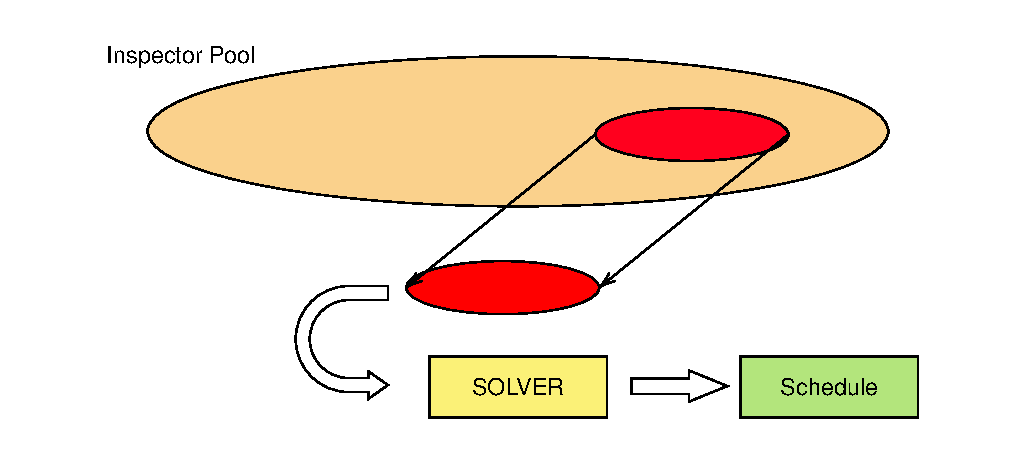
\includegraphics[scale=0.7]{iter1.pdf}
        \caption{First Iteration}
        \label{fig:my_label}
    \end{figure}
\end{frame}

\begin{frame}{Heuristic Solver: A Picture}
    \begin{figure}
        \centering
        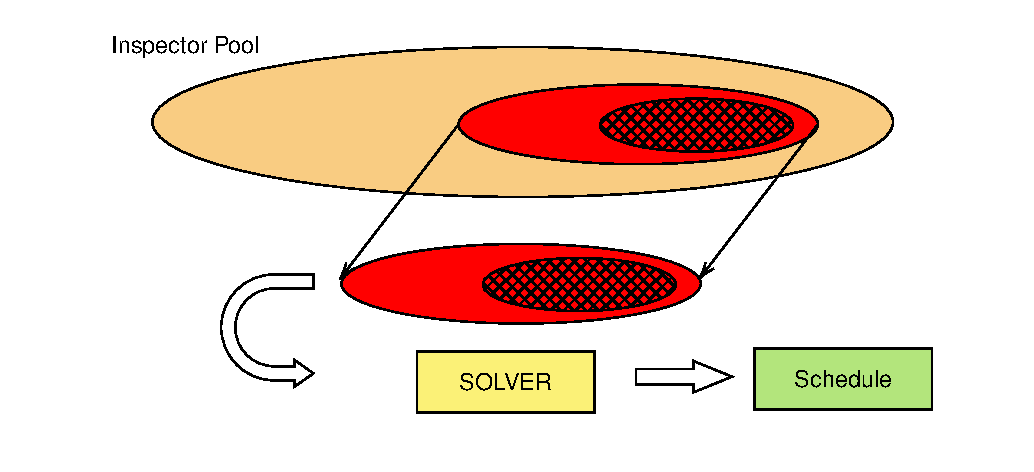
\includegraphics[scale=0.7]{iter2.pdf}
        \caption{Second Iteration}
        \label{fig:my_label}
    \end{figure}
\end{frame}

\begin{frame}{Heuristic Solver: A Picture}
    \begin{figure}
        \centering
        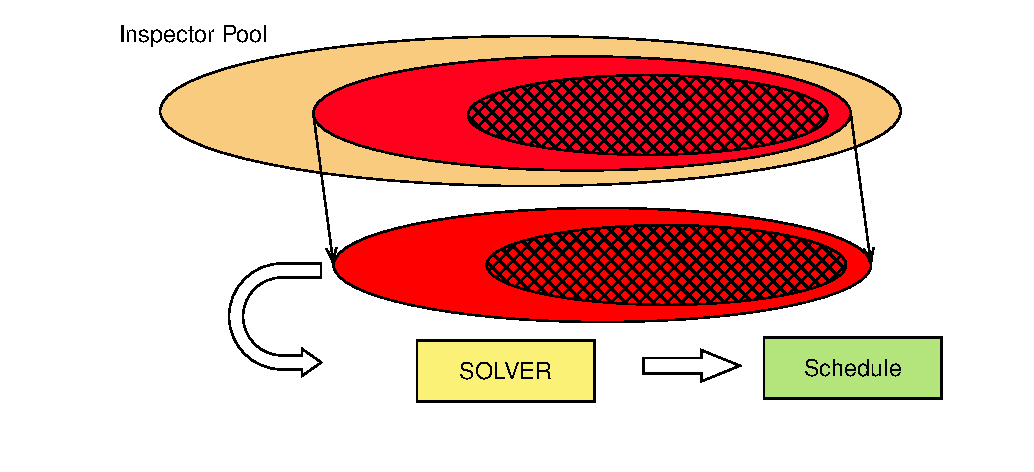
\includegraphics[scale=0.7]{iter3.pdf}
        \caption{Third Iteration}
        \label{fig:my_label}
    \end{figure}
\end{frame}

% \begin{frame}{Experiments}
% Experiment: Find the best 3 inspectors out of 6 inspector options, 1 at a time. $I = 6, n = 3, \Delta = 1$
% \begin{table}[h]
% \begin{tabular}{c|c}
%  iteration no. &  time taken to solve for 1 inspector (s) \\
%  \hline
%  1 & 487\\
%  2 & 142\\
%  3 & 29\\
% \end{tabular}
% \end{table}\\

% Experiment: Find the best 5 inspectors out of 10 inspector options, 1 at a time. $I = 10, n = 5, \Delta = 1$
% \begin{table}[h]
% \begin{tabular}{c|c}
%  iteration no. &  time taken to solve for 1 inspector (s) \\
%  \hline
%  1 & 531\\
%  2 & 304\\
%  3 & 102\\
%  4 & 229\\
%  5 & 211
% \end{tabular}
% \end{table}
    
% \end{frame}



% \begin{frame}{Conclusions}
%     \textbf{Conclusion}: the first iteration is the most time consuming and reducing the pool size for the first inspector is direction for future research.
% \end{frame}

% Hai, Ruby, Nate

\section{Challenges, Conclusion and Future Work}

\begin{frame}{Drawbacks}
   \textbf{Passenger Classification}
        \begin{itemize}
            \item No 'waiting' passenger counts
            \item No prior classification data
        \end{itemize}
       \textbf{Implementation}
        \begin{itemize}
            \item Run-time scales quickly with the number of inspectors
        \end{itemize}
    
\end{frame}

\begin{frame}{Further Work}
    \begin{itemize}
        \item \textbf{Alternative idea:} Since solving for 500 inspectors simultaneously is computationally expensive, consider turning the path constraint problem into a multiple-commodity flow problem for each base station and then decompose these flows into inspector paths.
        \item Not all 500 inspectors need to be used. What is the minimum number of inspectors needed to inspect sufficiently many passengers?
    \end{itemize}
\end{frame}

\begin{frame}{References}
    \bibliography{references}{}
    \bibliographystyle{plain}
\end{frame}

\begin{frame}{The End}
    \begin{figure}
        \centering
        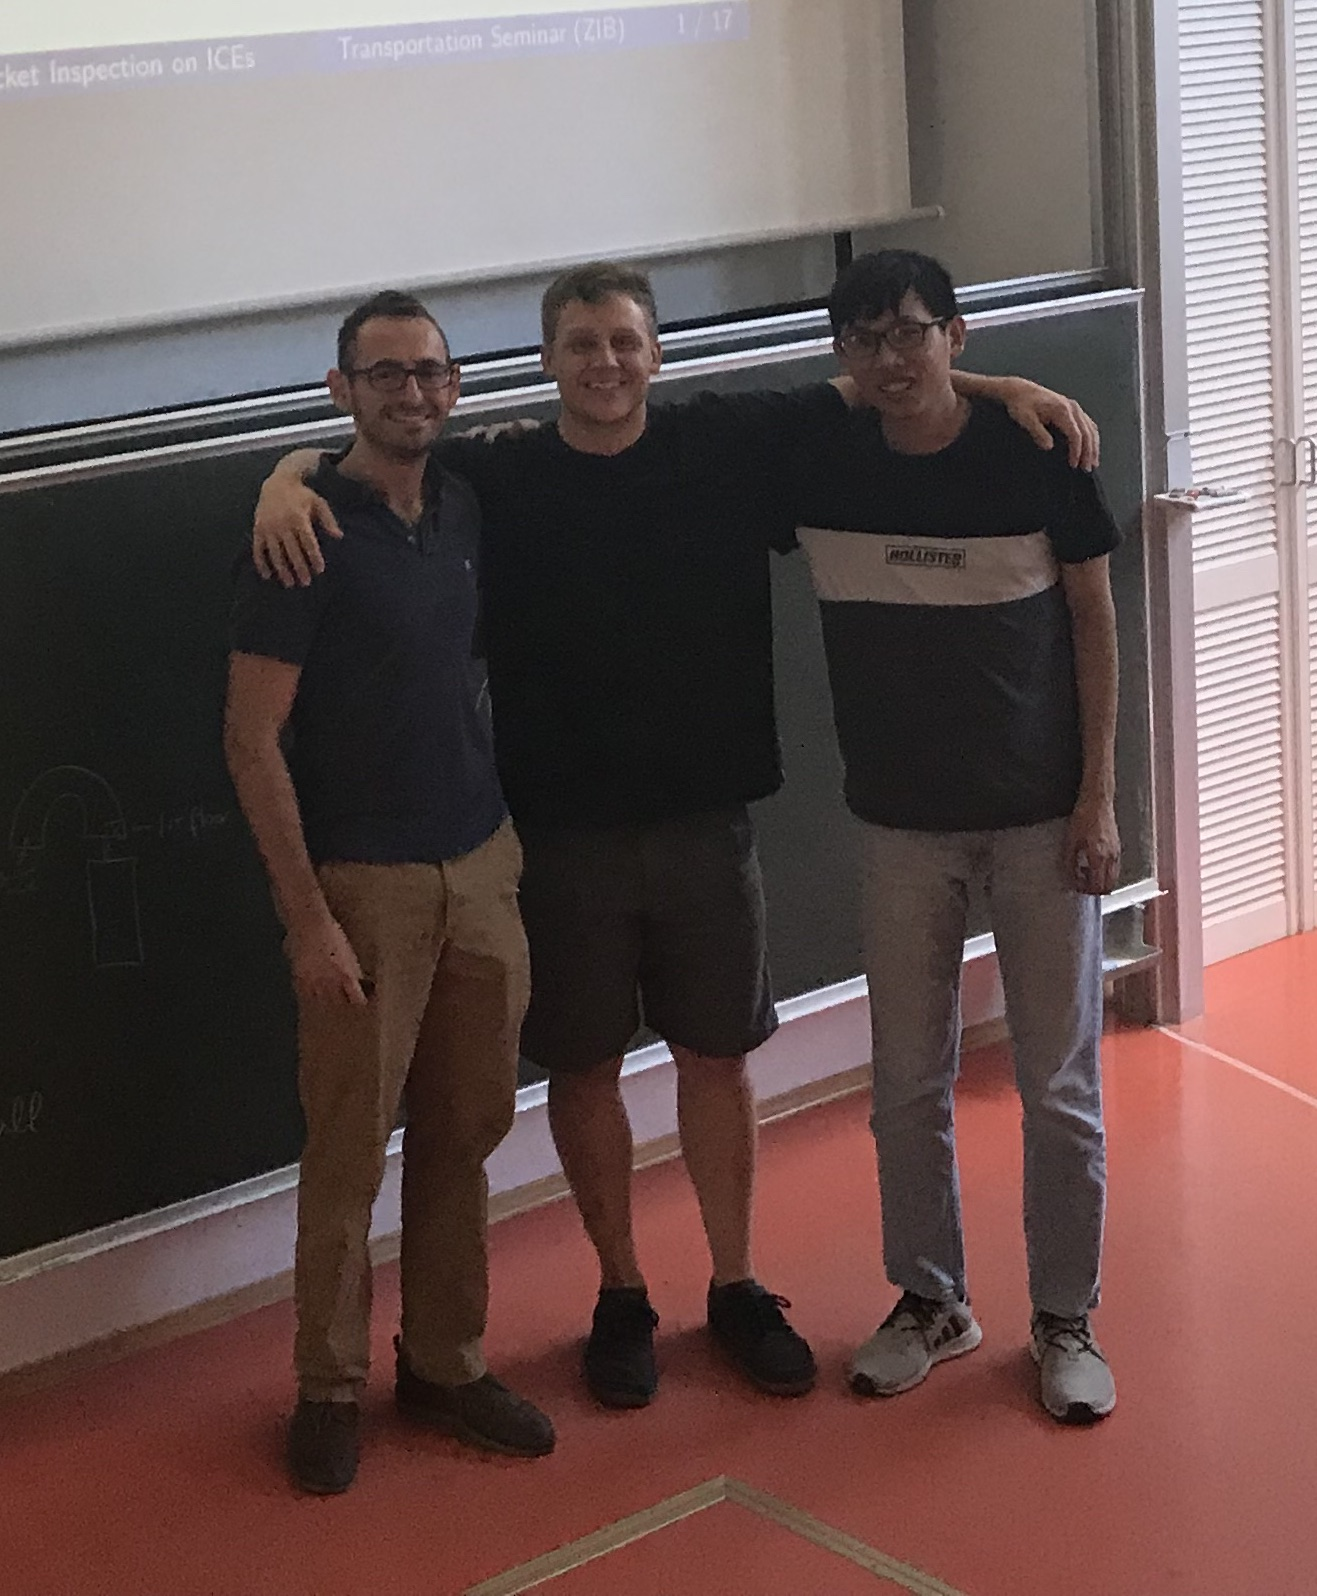
\includegraphics[scale=0.1]{team_DB_cropped.jpg}
        \caption*{Team DB}
        \label{fig:my_label}
    \end{figure}
    \centering
    \alert{Thank you!}
    
\end{frame}


\end{document}